\documentclass[9pt,letterpaper]{article}
%\usepackage[utf8]{inputenc}
\UseRawInputEncoding
\usepackage[english]{babel}
\usepackage{listings}
\usepackage{xcolor}
\usepackage{graphicx}

%For syntax highlighting
\definecolor{codegreen}{rgb}{0,0.6,0}
\definecolor{codegray}{rgb}{0.5,0.5,0.5}
\definecolor{codepurple}{rgb}{0.58,0,0.82}
\definecolor{backcolour}{rgb}{1,1,1}

%%Sets different parameters
\lstdefinestyle{mystyle}{
    backgroundcolor=\color{backcolour},   
    commentstyle=\color{codegreen},
    keywordstyle=\color{magenta},
    numberstyle=\tiny\color{codegray},
    stringstyle=\color{codepurple},
    basicstyle=\ttfamily\footnotesize,
    breakatwhitespace=false,         
    breaklines=true,                 
    captionpos=b,                    
    keepspaces=true,                 
    numbers=left,                    
    numbersep=5pt,                  
    showspaces=false,                
    showstringspaces=false,
    showtabs=false,                  
    tabsize=4
}
\lstset{style=mystyle}

\title{\textbf{Department of Computer Science and Engineering}}
\author{\textbf{Shivanirudh S G, 185001146, Semester VII }}

\date{30 September 2021}

\begin{document}
\maketitle
\hrule
\section*{\center{UCS1712 - Graphics and Multimedia Lab}}
\hrule 
\bigskip\bigskip

%Assignment name
\subsection*{\center{\textbf{Exercise 8: 3-Dimensional Projections in C++ using OpenGL}}}

%Objective
\subsection*{\flushleft{Aim:}}
\begin{flushleft}
    Write a menu driven program to perform Orthographic parallel projection and Perspective projection on any 3D object.
\end{flushleft}

%Code
\subsection*{\flushleft{Code:}}
\begin{flushleft}
\lstinputlisting[language = C++]{Headers.h}
\lstinputlisting[language = C++]{Signatures.h}
\lstinputlisting[language = C++]{Helpers.h}
\lstinputlisting[language = C++]{main.cpp}
\end{flushleft}
\newpage
\subsection*{\flushleft{Output:}}
\textbf{Orthographic projection:}\\

\begin{figure}[h]
    \centering
    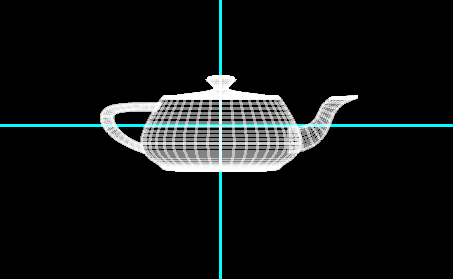
\includegraphics[height=5cm]{Outputs/OP1.png}
\end{figure}
\newpage
\textbf{Keyboard operations: }
\begin{figure}[h]
    \centering
    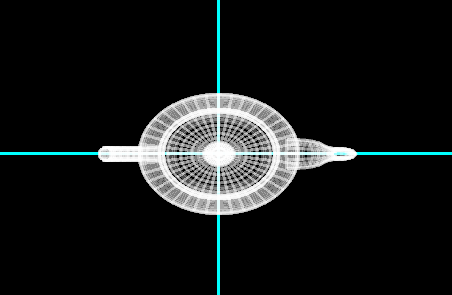
\includegraphics[height=5cm]{Outputs/OP2.png}
\end{figure}
\begin{figure}[h]
    \centering
    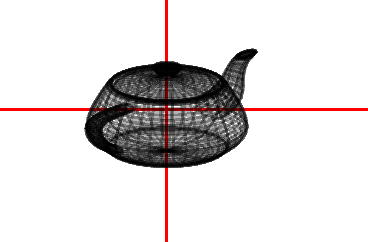
\includegraphics[height=5cm]{Outputs/OP3.png}
\end{figure}

\newpage
\textbf{Perspective projection:}\\

\begin{figure}[h]
    \centering
    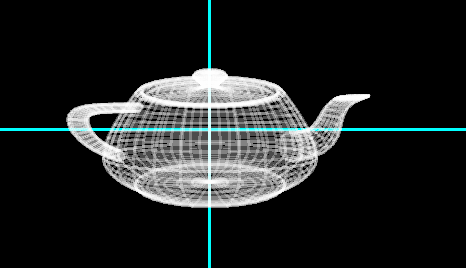
\includegraphics[height=5cm]{Outputs/OP4.png}
\end{figure}
\newpage
\textbf{Keyboard operations: }
\begin{figure}[h]
    \centering
    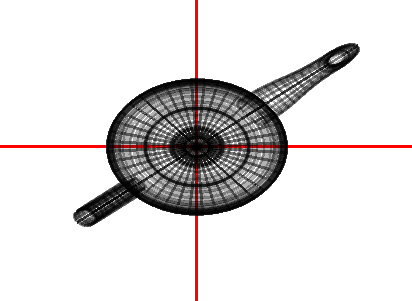
\includegraphics[height=5cm]{Outputs/OP5.png}
\end{figure}
\begin{figure}[h]
    \centering
    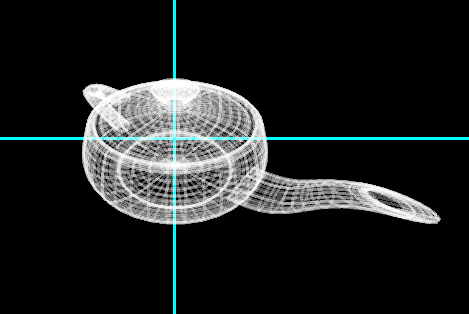
\includegraphics[height=5cm]{Outputs/OP6.png}
\end{figure}

\bigskip\bigskip
\hrule

\end{document}